\begin{figure}[htpb]
	\centering\capstart{}
	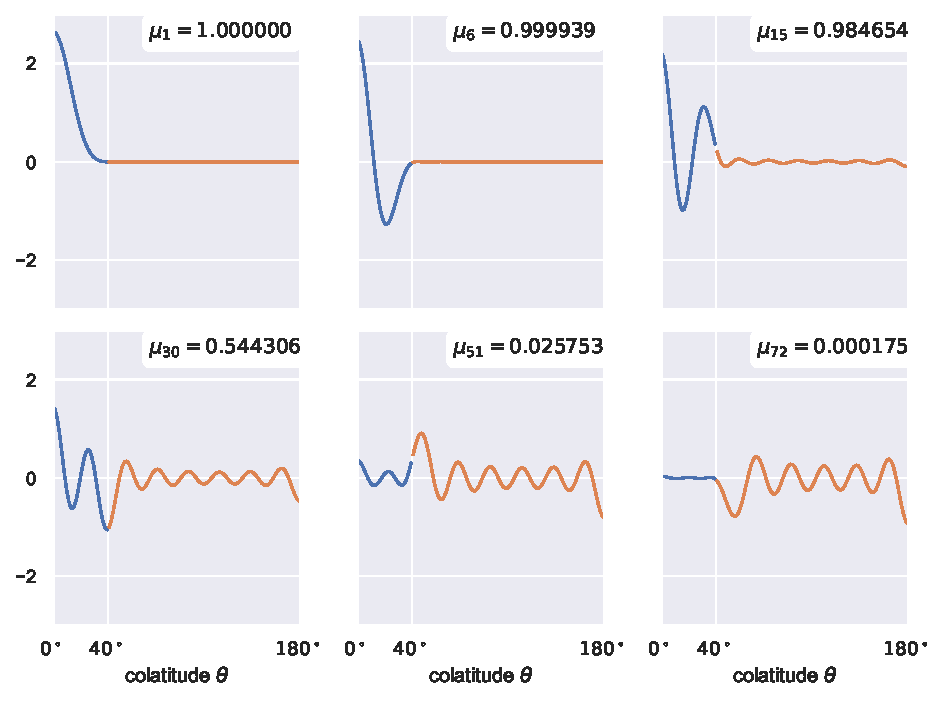
\includegraphics[width=\textwidth]{slepian_colatitude.pdf}
	\caption[
        The colatitudinal dependence of the polar cap Slepian functions
	]{
		The colatitudinal dependence of the three most-concentrated Slepian functions \(\pixel{\slepian{S}}\) within a polar cap of colatitudinal radius \(\SI{40}{\degree}\), \ie{} \(\alpha=1,2,3\), for a given order \(m=0,1,2,3\) shown left-to-right and top-to-bottom respectively.
		The bandlimit here is  \(L=16\), which corresponds to a Shannon number of \(N=30\).
		Blue curves show the concentration within the cap \(\SI{0}{\degree} < \theta < \SI{40}{\degree}\), whilst orange curves show the leakage into the rest of the sphere \(\SI{40}{\degree} < \theta < \SI{180}{\degree}\).
		The eigenvalue \(\mu\) quantifies the relative spatial concentration of the Slepian function, where lower values have increasing leakage in the orange curve.
	}\label{fig:chapter2_slepian_colatitude}
\end{figure}
